\documentclass[11pt,a4paper]{article}

\usepackage[T1]{fontenc}
\usepackage[utf8]{inputenc}
\usepackage{newtxtext,newtxmath}
\usepackage[margin=2.5cm]{geometry}
\usepackage{microtype}
\usepackage{graphicx}
\usepackage{booktabs}
\usepackage{tabularx}
\usepackage{caption}
\usepackage{xcolor}
\usepackage[round,authoryear]{natbib}
\usepackage[hidelinks]{hyperref}
\usepackage{setspace}

\captionsetup{font=small,labelfont=bf,labelsep=period}
\setstretch{1.08}
\graphicspath{{figures/}}

\newcommand{\sign}[1]{\textsf{#1}}

\title{\textbf{Measuring the Indus corpus before testing it:\\edition disagreement, near-copy leakage and detection limits}}
\author{Anonymous submission}
\date{}

\begin{document}
\maketitle

\begin{abstract}
\noindent Statistical and machine-learning work on the Indus script rests on a corpus of 2,270 distinct short texts. We measure three properties of this corpus that decide what such work can show. (1)~\emph{The editions disagree.} Matching 469 objects across the two standard transcriptions through the 1930s excavation registers, independently of their signs, we find that the editions read 12.9\% of signs differently (95\% CI 11.1--14.9\%; 14.0\% out of sample), and one text in three differs somewhere. (2)~\emph{Random splits leak.} Because moulded tablets and fixed formulae put near-copies of a text on different objects, a random split by object leaves a near-copy of 37\% of test texts in training even after exact repeats are removed (median of 200 splits; 95\% range 33--42\%), and of 62\% if they are not. (3)~\emph{Many questions lie below the detection limit.} Planted-answer controls show that a genre difference must exceed 0.57 bits per text to be found, that a relational reading of a joining sign needs about four times more texts, and that a widely used sign-order statistic passes on four of seven non-linguistic codes. We release a family-level split and a corrected concordance between the two sign lists, and recommend reporting practice for future quantitative work on the script.

\medskip
\noindent\textbf{Keywords:} Indus script; undeciphered writing; corpus reliability; data leakage; statistical power; ancient languages
\end{abstract}

\section{Introduction}

The Indus script was used in the Indus Valley in the third millennium BCE. No bilingual text is known and the language it records, if it records one, is unidentified \citep{parpola1994}. Quantitative study of the script began with the concordances of the 1960s and 1970s \citep{mahadevan1977} and now spans entropy arguments about whether the signs write language \citep{rao2009,sproat2014}, $n$-gram models of sign sequences \citep{yadav2010} and, as for other ancient corpora, neural models of restoration \citep{assael2022,sommerschield2023}.

This work treats the transcribed corpus as fixed and its texts as independent samples. Neither assumption holds, and the size of each departure has not been measured. We measure three quantities on which any quantitative claim about the script depends:

\begin{enumerate}
  \item \textbf{Agreement between editions} (Section~\ref{sec:editions}). If the two standard editions often read the same object differently, every result carries a reading error that is rarely reported.
  \item \textbf{Leakage under random splits} (Section~\ref{sec:leakage}). If test texts have near-copies in training, held-out scores partly measure memory. Leakage of this kind is a documented source of irreproducible results in machine-learning science \citep{kapoor2023} and in NLP benchmarks \citep{lewis2021,sogaard2021,lee2022}; it has not been measured for the Indus corpus.
  \item \textbf{Detection limits} (Section~\ref{sec:limits}). A null result is uninformative without the power of the test \citep{button2013}. We plant known answers in corpora of Indus size and record what standard tests recover.
\end{enumerate}

We make no claim about the meaning or sound of any sign, nor about any language. The results concern the corpus as a measuring instrument. Two of the errors we describe were first made in our own earlier analyses, and we report them as such.

\section{Related work}

\paragraph{Corpora and sign lists.} Two transcriptions are in general use: \citet{mahadevan1977} (M77), a concordance of 3,573 lines with its own sign list, and the Interactive Corpus of Indus Texts \citep[ICIT;][]{icit}, which follows the sign list of \citet{wells2015}. The two lists divide the sign repertoire differently, so comparing readings requires a concordance between them. To our knowledge, the rate at which the two editions disagree on the same objects has not been published.

\paragraph{Is it language?} \citet{rao2009} argued from conditional entropy that the sequences behave like language; \citet{farmer2004} had argued that the script is non-linguistic; \citet{sproat2014} showed that entropy-style statistics do not separate language from non-linguistic symbol systems. Section~\ref{sec:limits} extends Sproat's argument to a sign-order statistic.

\paragraph{Leakage.} Near-duplicate overlap between training and test sets inflates scores in question answering \citep{lewis2021} and language modelling \citep{lee2022}, and random splits can overstate performance relative to splits that respect structure in the data \citep{gorman2019,sogaard2021}. \citet{kapoor2023} catalogue leakage across scientific applications of machine learning. Ancient corpora are especially exposed, because formulae, stamps and moulds produce many near-identical texts.

\paragraph{Pre-registration.} We follow the practice of fixing analyses before outcomes are seen \citep{nosek2018}, adapted to a corpus that has been studied for decades and therefore cannot be treated as unseen.

\section{Data and procedures}
\label{sec:data}

\paragraph{Editions.} Our digital copy of M77 has 3,573 lines, 13,372 sign tokens and 417 signs, matching the published totals. ICIT has 5,679 inscriptions in reading order. About 90\% of ICIT comes from sites M77 already covers, so ICIT is mostly a second reading of the same objects rather than new data.

\paragraph{Distinct texts and families.} Moulded tablets repeat one text many times, so we count distinct sign sequences: M77 has 2,270. We join two distinct texts into one \emph{family} if they are within one sign edit of each other, or if one contains the other (for texts of three or more signs). The 2,270 texts form 1,477 families.

\paragraph{Procedures.} Every confirmatory test was written up before it was run, naming the statistic, the null distribution, the pass bar and the minimum sample. The write-up and its scripts were hashed (SHA-256) into a public file before any outcome was computed. Each positive result was then attacked by a separate analyst who wrote independent code without reading the original, and who pre-registered their own kill criteria. Section~\ref{sec:checks} reports one such attack.

\section{Agreement between the editions}
\label{sec:editions}

\subsection{Matching objects without their signs}

Comparing two editions requires pairs of readings known to belong to the same object. Matching texts by their signs would favour pairs that already agree. We therefore linked objects through the excavation registers of Mohenjo-daro, Harappa and Chanhu-daro \citep{mackay1938,vats1940,mackay1943}, by serial and field number. This yielded 469 objects: 342 seals, 81 tablets and 46 sealings.

Comparing readings also requires a concordance between the two sign lists. We built it from the 395 matched objects whose two readings have equal length, where the sign at each position can be compared without any concordance. Our first concordance contained errors: the five plain fish signs were cross-wired, one frequent sign was unmapped, and Mahadevan's practice of writing some signs twice where Wells has a single ``double'' sign had been scored as a substitution plus a missing sign. These errors had inflated the disagreement rate to 19.4\%. Appendix~\ref{app:concordance} lists the corrections. We report this because concordances between other sign lists are likely to contain similar errors, and because here they changed the result by a third.

\subsection{Result}

After correction the editions disagree on 12.9\% of compared signs (Table~\ref{tab:disagreement}). About one text in three is read differently somewhere.

\begin{table}[t]
\centering
\caption{Disagreement between M77 and ICIT on 469 register-matched objects, per compared sign. Intervals are 95\% text-bootstrap intervals.}
\label{tab:disagreement}
\begin{tabular}{lr}
\toprule
Kind of disagreement & Rate (95\% CI) \\
\midrule
Different sign & 7.3\% (6.1--8.6) \\
Sign present in one edition only & 5.0\% (3.8--6.3) \\
Adjacent signs in swapped order & 0.6\% (0.3--1.0) \\
\textbf{All kinds} & \textbf{12.9\% (11.1--14.9)} \\
\midrule
Texts with any difference & 34.5\% (30.3--38.8) \\
Texts read in opposite directions & 2.1\% (0.9--3.4) \\
\bottomrule
\end{tabular}
\end{table}

Disagreement is uneven (Figure~\ref{fig:disagreement}). Harappa objects disagree more than Mohenjo-daro objects (17.5\% against 10.8\%), and sealings more than tablets or seals (24\%, 18\% and 11\%). Signs that only M77 records lean towards the start of a text: 6.4\% of initial positions against 3.4\% of final and 2.8\% of medial ones. Nine of the twelve order swaps involve one sign, \sign{M328}, all on Harappa objects. Beyond these, there is no dominant error: the twenty most frequent disagreeing pairs account for only 24\% of disagreements.

\begin{figure}[t]
\centering
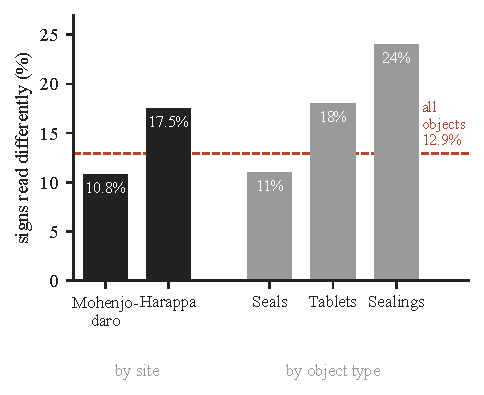
\includegraphics[width=0.62\textwidth]{fig1_disagreement}
\caption{Share of signs read differently by the two editions, by site and by object type, on register-matched objects. The dashed line is the rate over all 469 objects.}
\label{fig:disagreement}
\end{figure}

\subsection{Checks}
\label{sec:checks}

\paragraph{Fitting.} The corrections were derived from the same objects on which they are measured. An independent analyst re-derived them on half of the objects and measured on the other half, over 200 random halvings. The out-of-sample rate is 14.0\% (range 12.2--16.0\%). Fitting therefore lowers the estimate by about one point.

\paragraph{The fish pairing.} Of all 120 ways of pairing the five plain fish signs between the two lists, the corrected pairing gives the lowest disagreement (12.6\%); the next best gives 14.2\%, and the original pairing ranks 28th. The pairing rests on large counts, such as 37 of 38 and 22 of 23 same-position matches.

\paragraph{Alignment.} Across alignment costs and methods the rate ranges from 10.5\% to 13.2\%. The cut that rejects register links whose readings are too far apart matters more: random pairs pass it 11.6\% of the time, so it is needed, and keeping every register link gives 28\%, mostly from linking errors.

\paragraph{Beyond the register sample.} On 2,741 further M77 texts linked to ICIT by their signs, the rate is 11.0\%. This is a floor, because sign-based linking keeps pairs that agree: among register-matched pairs, those that sign-based linking would have admitted disagree on 8.6\% of signs, and those it would have missed on 67\%.

\subsection{Consequences for analysis}

The register-matched objects are the best-documented part of the corpus, so disagreement elsewhere is unlikely to be lower. Errors that both editors share are invisible to this comparison, since ICIT drew on M77 and on the same photographs.

To show how the rate bears on published claims, we re-ran nine structural findings on the signs both editions agree on, on the ICIT readings, and under noise that reproduces the measured pattern of disagreement (which signs are confused with which, where deletions fall, and how often texts are reversed). All nine pass at the measured rate. The weakest, that recurring sign pairs keep a fixed order, passes in only three of five runs when the noise is concentrated on rare signs. A finding about reading direction cannot be checked at all, because only eight left-to-right lines carry the same label and the same signs in both editions.

\section{Leakage under random splits}
\label{sec:leakage}

\subsection{How much random splits leak}

We drew 200 random splits of M77 by object, the usual practice, with about a fifth of objects in test, and counted test texts of two or more signs that have a copy in training. We did this twice: on all 3,424 texts, and after removing exact repeats first, as a careful modeller would, which leaves 2,263 texts. Without de-duplication, 39.1\% of test texts have an exact copy in training and 62.3\% a near-copy (95\% range 58.9--65.9\%). Removing exact repeats does not solve the problem: 37.3\% of test texts still have a near-copy in training (95\% range 33.3--41.6\%). The share depends on the copy rule and should always be reported with it (Figure~\ref{fig:leakage}); after de-duplication it ranges from 13.5\% for copies within one edit to 50.6\% for copies within two edits or contained.

\begin{figure}[t]
\centering
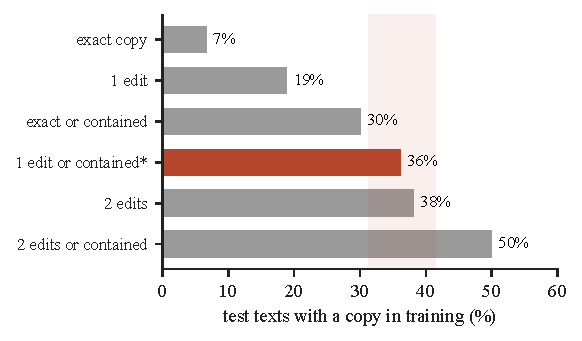
\includegraphics[width=0.62\textwidth]{fig2_leakage}
\caption{Share of test texts with a copy in training under random splits of M77 by object, by copy rule, on all texts and after exact repeats are removed. Bars are medians over 200 splits and whiskers 95\% ranges. The primary rule is marked with an asterisk.}
\label{fig:leakage}
\end{figure}

We made this error ourselves. Our first held-out set was drawn from distinct sequences at random, and 251 of its 554 texts (45\%) were within one edit of a development text. On that split, the real order of signs outscored every reordering in 63\% of held-out texts; without the leaked texts, in 42\%, against 3\% by chance. On a split by family the figure is 40.2\% against 5.7\% by chance. The finding survived, but not its original magnitude.

\section{Detection limits}
\label{sec:limits}

For each question below we planted a known answer, in Indus texts or in a real corpus thinned to Indus size, and recorded how often the test recovered it. Table~\ref{tab:limits} summarises the results.

\paragraph{Genres.} Unsupervised mixture models find a single genre in the Indus texts. Planting genres in 2,269 real texts shows that 80\% power requires a genre that differs by 0.57 bits per text in vocabulary, formula and length together. Object type, which a supervised classifier does separate on held-out texts, carries only 0.15 bits. A single genre is therefore expected even where registers exist. A contrast as strong as Mesopotamian seal legends against tags, 1.15 bits, would have been found.

\paragraph{A joining sign as a relation word.} One frequent sign often stands between two sign groups. If it meant something like ``son of'', the groups on either side should also occur as independent texts more often than chance. Before applying the test to Indus data, we ran it on real Ur~III and Old Babylonian seal legends thinned to Indus size. It recovered ``son of'' in 3 and 0 of 100 samples respectively, against a bar of 80; on the full 5,180 Ur~III legends it ranks ``son of'' first. We therefore did not run the test on Indus data. It needs about four times more texts.

\paragraph{A sign enriched on pottery.} A test of whether the jar-shaped sign marks vessels has 47\% power on the 65 pottery texts from Harappa, Lothal and Kalibangan on which both editions agree. About 250 are needed.

\paragraph{Language or code.} Whether the script writes language is the most debated statistical question about it \citep{farmer2004,rao2009,sproat2014}. We tested two approaches against known cases. The first is a sign-order statistic: the share of texts whose real order outscores every reordering of their own signs, under a bigram model trained on development texts. Indus scores 0.40. Run unchanged on seven non-linguistic codes and six writing systems, each sampled to Indus size and split by family, it ranges from 0.98 for weather reports to 0.10 for short Latin inscriptions (Figure~\ref{fig:order}). Four of the seven codes pass the pre-registered bar of 0.30. The statistic detects fixed formats, not language, which extends \citeauthor{sproat2014}'s \citeyearpar{sproat2014} argument from entropy measures to order. The second approach, a classifier trained on known languages and codes, reaches a balanced accuracy of 0.61 when each code is held out in turn, and 0.69 on genre-matched short labels, against a pre-registered gate of 0.80. Neither approach can answer the question at this corpus size.

\begin{figure}[t]
\centering
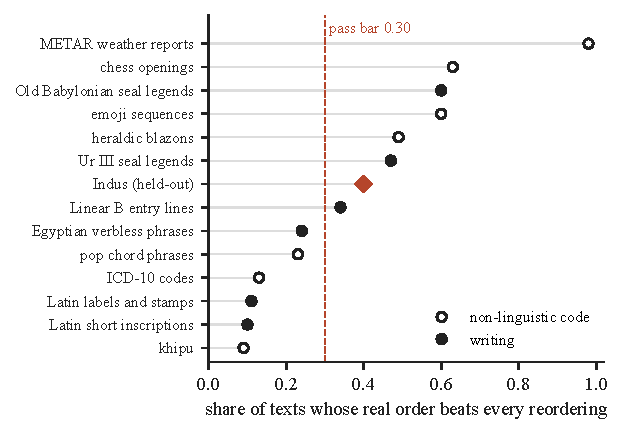
\includegraphics[width=0.62\textwidth]{fig4_order}
\caption{The sign-order statistic on Indus and on writing systems and non-linguistic codes sampled to Indus size and split by family (median of five seeds). Four of seven codes pass the bar that Indus passes.}
\label{fig:order}
\end{figure}

\begin{table}[t]
\centering
\caption{Detection limits at the present corpus size.}
\label{tab:limits}
\begin{tabularx}{\textwidth}{lXX}
\toprule
Question & What the test needs & What the corpus has \\
\midrule
Distinct genres & A difference of 0.57 bits per text & Object type differs by 0.15 bits \\
Joining sign as relation word & About four times more texts & 2,270 distinct texts \\
Jar sign enriched on pottery & About 250 pottery texts & 65 \\
Language against code & A statistic that separates known cases & None passed its gate \\
\bottomrule
\end{tabularx}
\end{table}

Some of these limits will move with new data. The third volume of the \emph{Corpus of Indus Seals and Inscriptions}, not yet available in a digital corpus we could use, and excavation databases of marked sherds could bring the pottery question within reach. We have hashed forward predictions for such data so that the test is fresh when it arrives.

\section{Recommendations}

For quantitative work on the Indus corpus we recommend that authors:
\begin{enumerate}
  \item state which edition is used, and report key results on both editions or under noise matched to the measured disagreement;
  \item split by near-copy family rather than by object or by text, and report the copy rule and the leaked share of any split used;
  \item report the power of any test whose result is null, using planted answers in a corpus of Indus size;
  \item validate any statistic offered as evidence of language on non-linguistic codes of matching size and format.
\end{enumerate}

\section{Limitations}

\paragraph{Shared errors.} Disagreement between the editions is a lower bound on reading error, because errors shared by both are invisible.

\paragraph{One sign list.} All tests run in Mahadevan's sign numbering. The main structural tests were also run under twelve alternative sign lists, but the leakage figures reported here use M77 and are likely to rise under sign lists that merge similar signs.

\paragraph{Simulators.} The planted-answer controls write real languages in invented scripts. They may differ from Indus texts in, for example, how often names occur, which affects the size of the limits in Section~\ref{sec:limits}.

\paragraph{Analysis by AI agents.} Most analyses and all independent attacks were carried out by AI agents working under written rules, with a human lead who set the questions and reviewed the findings. Pre-registration and hashing limit what an agent could adjust after seeing data. The attacking agents share a model family with the original analysts, so their independence is partial, and none of this replaces review by epigraphers.

\section*{Data and code availability}

Code, pre-registrations with their hashes, results files and a ledger of every test run are available in the project repository [URL withheld for review]. The family-level split is released as text numbers with its hash, and the corrected concordance with the evidence for each entry. The corpus files are not redistributed, because neither source states terms that permit it; a script rebuilds them from the public sources.

\section*{Use of AI}

AI agents performed most analyses, independent attacks and drafting, as described under Limitations. The human author set the research questions and directed and reviewed the work. Reported numbers were checked against their results files by an automated script and by agent review.

\section*{Competing interests and funding}

None declared. The work received no external funding.

\bibliographystyle{plainnat}
\bibliography{refs}

\appendix
\section{Corrections to the sign-list concordance}
\label{app:concordance}

\begin{table}[h]
\centering
\caption{Corrections to the M77--Wells concordance, with same-position matches on equal-length register-matched readings.}
\begin{tabular}{lll}
\toprule
M77 sign & Wells sign & Evidence \\
\midrule
\sign{M65} (plain fish) & \sign{W235} & 22 of 23 \\
\sign{M67} (plain fish) & \sign{W240} & 37 of 38 \\
\sign{M70} (plain fish) & \sign{W231} & 9 of 9 \\
\sign{M72} (plain fish) & \sign{W233} & 20 of 23 \\
\sign{M66} (ticked fish) & \sign{W236} & 3 of 3 \\
\sign{M389} & \sign{W806} & 14 of 18 \\
\sign{M245} written twice & \sign{W617} (one sign) & doubled-sign convention \\
\sign{M176} written twice & \sign{W401} (one sign) & doubled-sign convention \\
\sign{M375} written twice & \sign{W792} (one sign) & doubled-sign convention \\
\bottomrule
\end{tabular}
\end{table}

Three one-to-many entries were also narrowed (\sign{M162}, \sign{M216}, \sign{M387}). The remaining ticked fish (\sign{M68}, \sign{M71}, \sign{M73}) were assigned by analogy with the plain fish and are unverified on matched objects.

\end{document}
